\chapter{Задача Коши для волнового уравнения в $\mathbb{R}^2$ и $\mathbb{R}^3$ . Энергетическое неравенство. Единственность решения задачи Коши.}
\label{cha:6}

\textbf{Напоминание}

\begin{enumerate}
	\item \blue{формула Гаусса-Остроградского}
		$$\underset{\Omega}{\overset{}{\iint}} \frac{\partial w}{\partial x_i} d \overline{x} = \underset{\partial \Omega}{\overset{}{\oint}} w \cdot n_i \cdot d \sigma$$
	\item \blue{формула интегрирования по частям}\\
		$$\begin{gathered}
			w = f \cdot g, \; \underset{\Omega}{\overset{}{\iint}} (\frac{\partial f}{\partial x_i} g + \frac{\partial g}{\partial x_i} f) d \overline{x} = \underset{\partial \Omega}{\overset{}{\oint}}  f \cdot g \cdot n_i d \sigma \; \Rightarrow \\
			\Rightarrow \; \underset{\Omega}{\overset{}{\iint}} \frac{\partial f}{\partial x_i} g d \overline{x} = \underset{\partial \Omega}{\overset{}{\oint}} f \cdot g \cdot n_i d\sigma - \underset{\Omega}{\overset{}{\iint}} \frac{\partial g}{\partial x_i} \cdot f d \overline{x}
		\end{gathered}$$
	\item \blue{теорема о потоке}
		$$\begin{gathered}
			w = \frac{\partial f}{\partial x_i}, \; \underset{\Omega}{\overset{}{\iint}} \frac{\partial^2 f}{\partial x_i^2} \cdot d \overline{x} = \underset{\partial \Omega}{\overset{}{\int}} \frac{\partial f}{\partial x_i} \cdot n_i d\sigma \text{ - суммируем по } i: \\
			\underset{\Omega}{\overset{}{\iint}} \triangle f d \overline{x} = \underset{\partial \Omega}{\overset{}{\oint}} (\overline{\nabla} f, n) d\sigma = \underset{\partial \Omega}{\overset{}{\oint}} \frac{\partial f}{\partial \overline{n}} d\sigma
		\end{gathered}$$
	\item \blue{производная интеграла по параметру}
		$$F(t) = \underset{a(t)}{\overset{b(t)}{\int}}h(t,x) dx, \; F'(t) = \underset{a(t)}{\overset{b(t)}{\int}}\frac{\partial h}{\partial t} (t,x) dx + h(t, b(t)) \cdot b'(t) - h(t, a(t)) \cdot a'(t)$$
\end{enumerate}

\textbf{Волновое уравнение}
$$u_{tt} = a^2 \triangle_{\overline{x}} u = a^2 (u_{x_1 x_1} + \dots + u_{x_n x_n})$$
Рассмотрим задачу Коши для волнового уравнения:
$$\begin{cases}
	u_{tt} = a^2 \triangle_{\overline{x}} u, \; t > 0, \; x \in \mathbb{R}^n \\
	\left.
  		\begin{array}{ccc}
    		u|_{t=0} = \varphi(x) \\
    		u_t |_{t=0} = \psi (x)
  		\end{array}
	\right\}, \; \overline{x} \in \mathbb{R}^n
\end{cases}$$

Рассмотрим случай \red{n = 2}: 
$$\begin{gathered}
	u_{tt} - a^2 (u_{x_1 x_1} + u_{x_2 x_2}) = 0 \\
	A(\lambda, \mu_1, \mu_2) = \lambda^2 - a^2 (\mu_1^2 + \mu_2^2) \text{ - характеристический многочлен} \\
	\overline{n} = (n_t, n_1, n_2), \; A(\overline{n}) = (n_t)^2 - a^2 (n_1^2 + n_2^2) = 0
\end{gathered}$$
Т.о. характеристической поверхностью является конус:
\begin{figure}[h]
	\begin{multicols}{2}
		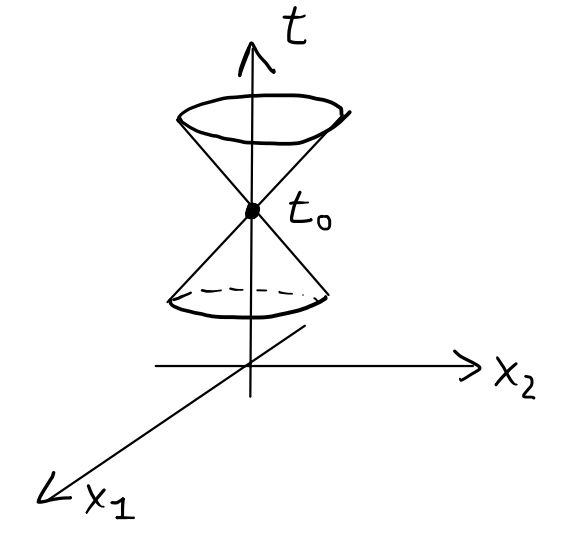
\includegraphics[width=70mm]{cha6im1}
		\columnbreak
		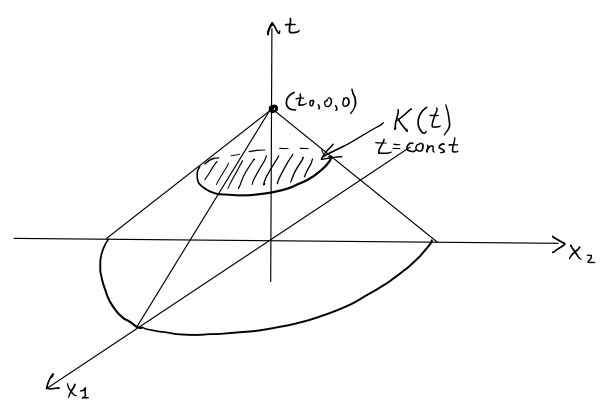
\includegraphics[width=110mm]{cha6im2}
	\end{multicols}
\end{figure} 

Получаем уравнение:
$$a^2 (t_0 -t)^2 = x_1^2 + x_2^2, \; a^2 (t_0 - t)^2 - (x_1^2 + x_2^2) = 0 = F(t, x_1, x_2)$$
Нормаль к конусу:
$$\overline{n} = (F_t, F_{x_1}, F_{x_2}) = (2a^2(t- t_0), -2x_1, -2x_2) = 2(a^2(t-t_0), -x_1, -x_2)$$
Получаем уравнение характеристик:
$$a^4 (t-t_0)^2 - a^2 (x_1^2 + x_2^2) = 0$$
\begin{definition}\label{lec:6/def:1}
	\blue{Интегралом энергии} называется величина
	$$E(t) := \frac{1}{2} \underset{K(t)}{\overset{}{\varoiint}}\left[ (u_t)^2 + a^2 \left( (u_{x_1})^2 + (u_{x_2})^2 \right)^2 \right] d \overline{x} = \frac{1}{2} \underset{|\overline{x}| \le a (t_0 - t)}{\overset{}{\varoiint}}\left[ (u_t)^2 + a^2 \left| \overline{\nabla_x} u \right|^2 \right] d \overline{x}$$
\end{definition}

\begin{theorem}[\red{Энергетическое неравенство}]\label{lec:6/the:1}
	Пусть $u(t,x)$ удовлетворяет волновому уравнению в конусе $\Omega$. Тогда: 
	$$\forall t_1, t_2 \in (0, t_0), t_1 < t_2: \; E(t_1) \ge E(t_2)$$
\end{theorem}
\begin{Proof}
	Хотим показать, что $E(t)$ убывает по $t$. Идея доказательства состоит в том, чтобы рассмотреть $E'(t)$ и показать, что она $\le 0$.\\
	Запишем $E(t)$ в следующем виде:
	$$E(t) = \frac{1}{2} \underset{0}{\overset{a(t_0-t)}{\int}}\underset{|\overline{x}| = \tau}{\overset{}{\oint}}\left[ (u_t)^2 + a^2 \left( (u_{x_1})^2 + (u_{x_2})^2 \right)^2 \right] d \sigma d \tau$$
	Найдем производную:
	$$\begin{gathered}
		E'(t) = \frac{2}{2}\underset{K(t)}{\overset{}{\varoiint}} \left[ u_t u_{tt} + a^2 (u_{x_1} u_{x_1 t} + u_{x_2} u_{x_2 t}) \right] d \overline{x} - \frac{a}{2} \underset{|\overline{x}| = a(t_0 - t)}{\overset{}{\varoiint}}\left[ (u_t)^2 + a^2 \left| \overline{\nabla_x} u \right|^2 \right] d \sigma = \\
		= \underset{K(t)}{\overset{}{\varoiint}} u_t \triangle u d \overline{x} + a^2 \Bigg[ \underset{|\overline{x}| = a(t_0 - t)}{\overset{}{\varoiint}} (u_{x_1} u_{x_1} n_1 + u_{x_2} u_{x_2} n_2) d \sigma - \\
		- \underset{K(t)}{\overset{}{\varoiint}} (u_{x_1 x_1} u_t + u_{x_2 x_2} u_t) d \overline{x} \Bigg] - \frac{a}{2} \underset{|\overline{x}| = a(t_0 - t)}{\overset{}{\varoiint}}\left[ (u_t)^2 + a^2 \left| \overline{\nabla_x} u \right|^2 \right] d \sigma \\
		(\text{применили формулу интегрирования по частям для } f = u_t \text{ и } g = u_{x_1})
	\end{gathered}$$
	Таким образом получаем:
	$$\begin{gathered}
		E'(t) = -\frac{a}{2} \underset{|\overline{x}| = a(t_0 - t)}{\overset{}{\varoiint}}\Big[ (u_t)^2 + a^2 (u_{x_1})^2 (n_1^2 + n_2^2) + a^2 (u_{x_2})^2 (n_1^2 + n_2^2) + \\
		+ a^2 (u_{xx})^2 (n_1^2 + n_2^2) - 2 a u_t u_{x_1} n_1 - 2 a u_t u_{x_2} n_2\Big] d \sigma = -\frac{a}{2} \underset{|\overline{x}| = a(t_0 - t)}{\overset{}{\varoiint}}\Big[ a^2 (u_{x_1})^2 n_2^2 + \\
		+ a^2 (u_{x_2})^2 n_1^2 - 2 a^2 u_{x_1} u_{x_2} n_1 n_2 + (u_t - a u_{x_1} n_1 - a u_{x_2} n_2)^2\Big] d \sigma = \\
		= -\frac{a}{2} \underset{|\overline{x}| = a(t_0 - t)}{\overset{}{\varoiint}}\Big[(u_t - a u_{x_1} n_1 - a u_{x_2} n_2)^2 + (a u_{x_1} n_2 - a u_{x_2} n_1)^2 \Big] d \sigma \le 0
	\end{gathered}$$
	Т.е. $E'(t) \le 0$ (не возрастает), что и требовалось доказать.
\end{Proof}

\begin{conseq}[]\label{lec:6/the:1}
	Решение задачи Коши единственно.
\end{conseq}
\begin{Proof}
	Имеем задачу Коши:
	$$\begin{cases}
		u_{tt} = a^2 \triangle u, \; t > 0, \; x \in \mathbb{R}^n \\
		\left.
	  		\begin{array}{ccc}
	    		u|_{t=0} = \varphi(x) \\
	    		u_t |_{t=0} = \psi (x)
	  		\end{array}
		\right\}, \; \overline{x} \in \mathbb{R}^n
	\end{cases}$$
	Предположим, что существует два различных решения $u_1$ и $u_2$. Рассмотрим их разность $z = u_1 - u_2$, для нее задача Коши имеет вид:
 	$$\begin{cases}
		z_{tt} = a^2 \triangle z, \; t > 0, \; z \in \mathbb{R}^n \\
		\left.
	  		\begin{array}{ccc}
	    		z|_{t=0} = 0 = z (0, x_1, x_2) \\
	    		z_t |_{t=0} = 0
	  		\end{array}
		\right\}, \; \overline{x} \in \mathbb{R}^n
	\end{cases}$$
	$$\begin{gathered}
		E(t) = \underset{K(t)}{\overset{}{\varoiint}} \left[ (z_t)^2 + a^2 \left( (z_{x_1})^2 + (z_{x_2})^2 \right)^2 \right] d \overline{x} \\
		E(0) = \underset{K(0)}{\overset{}{\varoiint}} \left[ (z_t)^2|_{t=0} + a^2 \left( (z_{x_1})^2 + (z_{x_2})^2 \right)^2|_{t=0} \right] d \overline{x} = 0 \\
		\text{(из начальных условиях задачи Коши)}
	\end{gathered}$$
	Из энергетического неравенства имеем: $\forall t: E(t) \le E(0) = 0$. Тогда получаем, что $E(t) \equiv 0 \; \Rightarrow \; z_t \equiv z_{x_1} \equiv z_{x_2} \equiv 0 \; \Rightarrow \; z \equiv 0$. Т.к. $z|_{t=0} = 0$, то $z \equiv 0 \; \Rightarrow \; u_1 \equiv u_2$.
\end{Proof}

